\documentclass[12pt,a4paper]{article}
\usepackage[margin=25mm]{geometry}

\usepackage{titlesec}
\usepackage[toc,page]{appendix}
\usepackage{graphicx}
\usepackage{hyperref}

\graphicspath{ {./images/} }

\hypersetup{
    colorlinks=true,
    linkcolor=blue,
    filecolor=blue,      
    urlcolor=blue,
}
\setcounter{secnumdepth}{4}
%\usepackage{indentfirst}

\titleformat{\paragraph}
{\normalfont\normalsize\bfseries}{\theparagraph}{1em}{}
\titlespacing*{\paragraph}{0pt}{3.25ex plus 1ex minus .2ex}{1.5ex plus .2ex}


\begin{document}

\begin{titlepage}
	\centering
	{\scshape\LARGE McMaster University \par}
	\vspace{2cm}
	{\scshape\Large Project Deliverable \#4 \par}
	\vspace{4cm}
	{\huge\bfseries EMG Capturing Software\par}
	\vspace{2cm}
	{\Large\itshape by Marato Gebremichael\par}
	
	\vfill
	Course: 3RQ3 – Software Requirements and Specifications\par
    Instructor: Sean Watson

	\vfill

% Bottom of the page
	{\large \today\par}
\end{titlepage}

\tableofcontents

\newpage

\listoftables

\listoffigures

\newpage

\section{Introduction}

\indent This application will be designed to interface, capture and analyze electromyography (EMG) signals from a portable EMG device. 
EMG signals are biomedical signals that measure the muscle fiber potential (muscle action). 
These signals can be used for diagnosing muscle response for both medical and fitness purposes \cite{Mayo Clinic}.

\section{Description}

\subsection{Definitions}

\begin{table}[htbp]
	\centering
	
	\begin{tabular}{p{0.35\linewidth}p{0.6\linewidth}}
		\textbf{Noun}  & \textbf{Definition} \\
		
		Electromyography (EMG) & diagnostic procedure to assess the health of muscles and the nerve cells that control them (motor neurons) \\
		EMG signal             & biomedical signal that measures electrical currents generated in muscles during its contraction representing neuromuscular activities \\
		USB (Universal Serial Bus) & industry protocol for communication and power transfer from device to device  \\
		BT (Bluetooth) & industry wireless protocol for communication between devices \\
		Filter (signal processing)     & method for removing unwanted components of a signal and highlighting wanted components     \\

	\end{tabular}
	\textbf{\caption { Definitions }}
\end{table}

\subsection{System outline}

The application will be composed of a graphical user interface that contains a suite of controls to manage and 
display the capturing of the data from the EMG device. The application will display data as it's being captured as well as provide the user with the option to save and recall the data for offline analysis.

\subsection{Users}

The end-users of the application will include:

\begin{itemize}
	\item Private customer
	\item Trainer
	\item Nurse
	\item Doctor
\end{itemize}

\subsection{Owners}

The owners and maintainers of the application will include:

\begin{itemize}
	\item Private customer (ex. a fitness practitioner or private clinic)
	\item Hospital
	\item Software company
\end{itemize}

The maintenance including bug fixes will be completed via automatic software updates. 

\subsection{Use Case Diagrams}

\begin{figure}[h]
	\centering
	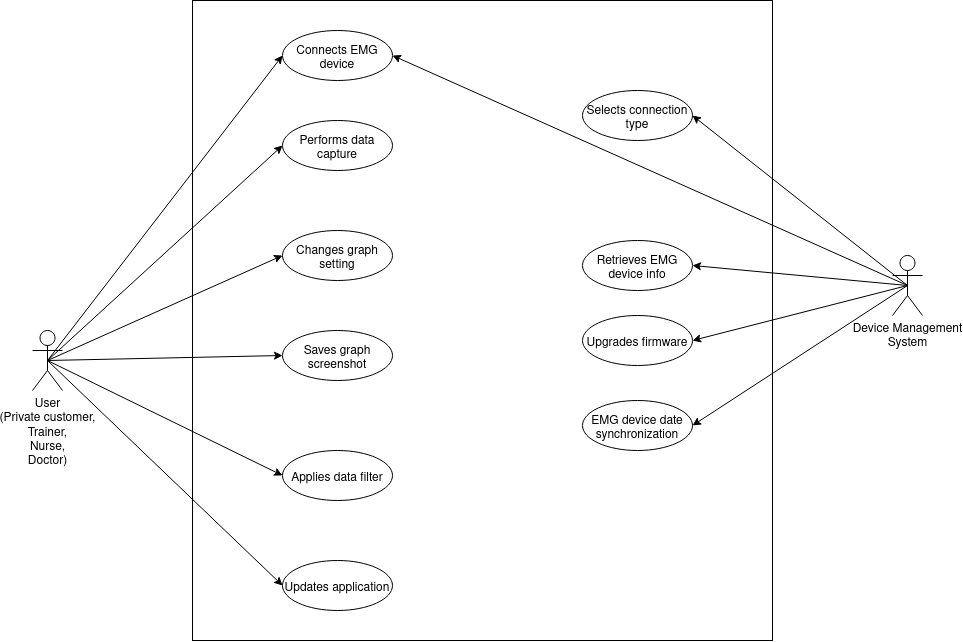
\includegraphics[scale=0.40]{Project Use Case Diagram.png}
	\caption{Use Case Diagram}
	\label{Data Classes}
\end{figure}

\newpage

\section{Constraints}

\begin{itemize}
	\item The application must be available on both Windows and Mac operating systems
	\item The application must interface existing EMG devices on the market, few devices include:
	
		\begin{itemize}
			\item Roam NXT by Laborie company
			\item Goby IV by Laborie company
			\item Solar Blue by MMS company
		\end{itemize}

	\item Application host device must be connected to the internet for software updates
\end{itemize}

\newpage

\section{System features}

\subsection{Menu bar}

The application must feature a menu bar from which common menu items will be available such as: help, settings, file open/close etc.

\subsubsection{Status bar}

The application must feature a status bar where information regarding the EMG device such as: connection type, connection status and device serial number.

\subsubsection{Closing the application}

The user shall be alerted if attempting to close the application during a capturing session.

\subsubsection{Out of range data}

The user shall be notified if the captured data falls out of range of the current graph setting.

\subsection{Data capture}

The application shall be able to capture the EMG signal from the device and save it onto the host of application.

\subsubsection{Device connection methods}

The device capture should be made via the following two means of device connection:

\begin{itemize}
	\item Wired - via USB connection
	\item Wireless - via Bluetooth connection
\end{itemize}

\subsubsection{Data capture properties}

\begin{table}[htbp]
	\centering
	\begin{tabular}{|l|l|}
		\hline
		\textbf{Property}  & \textbf{Limits} \\
		\hline
		Number of channels & up to 2 channels of EMG data\\
		\hline
		Signal amplitude & +/- 10mV \\
		\hline
		Signal bandwidth & 1Hz to 5000Hz \\
		\hline
	\end{tabular}
\end{table}

\subsubsection{Data capture length}

The application shall be able to continuously capture up to 1 hour of data.

\subsubsection{Live data capture}

The application shall capture the live EMG signal form the connected device and display on the graph.

\subsubsection{Data saving}

The user shall be able to save the raw captured data in (.csv) format along with information about the application version and EMG device (hardware/firmware version and serial number).

\subsubsection{Data recall}

The user shall be able to recall up to two saved captured data in (.csv) format simultaneously and display it on a single graph.

\subsection{Filter library}

The application shall feature filters implemented using an internal library for noise and data filtering.

\subsubsection{Filtering method}

The filters shall be able to run in real-time as the data is being captured by the application. 
The filters shall also be able to be applied during on data that was recalled.

\subsubsection{Noise filtering}

The application shall be able to filter DC to low frequency noise ($<$ 100Hz) and high frequency noise ($>$ 5000Hz). \\

The following are some critical unwanted signals to filter: 

\begin{itemize}
	\item Signals ($<$ 100Hz): 50/60Hz electrical utility frequency signals
	\item Signals ($>$ 5000Hz): AM/FM radio signals
\end{itemize}

Refer to following link for more signal types: \cite{ICGC} \href{https://www.ic.gc.ca/eic/site/smt-gst.nsf/eng/sf10759}{Canadian Table of Frequency Allocations}

\subsubsection{Data filtering}

The following filters shall be made available to be applied on the captured data:

\begin{itemize}
\item moving average - running average filter to smoothen the data 
\item peak - filter to highlight the peaks of a signal
\item low-pass filter - filter to remove signal components beyond a certain cut-off frequency
\item high-pass filter - filter to remove signal components below a certain cut-off frequency
\end{itemize}

\subsection{Graph settings}

The user shall be able to select the following settings of the graph:

\begin{itemize}
\item Horizontal scale (time measured in seconds)
\item Vertical scale (amplitude measured in millivolts)
\item Grid scale 
\item Adding and removing of x and y markers
\item Background color of the graph
\item Color of the grid
\item Color of the trace (data)
\item Color of the markers
\end{itemize}


\subsubsection{Data navigation}

The user shall be able to navigate the data along the time axis from start to finish.

\begin{table}[htbp]
	\centering
	\begin{tabular}{|c|l|l|}
		\hline
		\textbf{Capture Complete} & \textbf{Graph mode}  & \textbf{Navigation type} \\
		\hline
		Yes & User view mode & Able to use navigation bar\\
		\hline
		No & Real time capture & Navigation bar disabled \\
		\hline
	\end{tabular}
\end{table}


\subsubsection{Graph screenshot}

The user shall be able to save the current screenshot of graph to a (.png) image format on the application host via a button.

\newpage

\section{Interface}

\subsection{Connecting to an EMG device}

The application shall allow the user to connect to an existing two channels EMG device.

\subsubsection{Connection type}

The application shall allow the user to connect to an EMG device via:

\begin{itemize}
\item Wired connection
\item Wireless
\end{itemize}

\subsubsection{Retrieving device information}

The application shall allow the user to retrieve EMG device information such as: 

\begin{itemize}
\item device local time
\item battery status
\item firmware version
\item hardware version
\item serial number
\end{itemize}

\subsubsection{Firmware upgrade}

The application shall be able to complete firmware updates automatically if available.

\subsubsection{Date synchronization}

The application shall automatically synchronize the EMG device local time with the local time of the application.

\newpage

\section{Quality attributes}

\subsection{User Interface}

The application shall have an intuitive interface with support for a touch screen interface.

\subsubsection{Application graph}

The application shall feature a graph that takes up majority of the screen on the main page.

\subsubsection{Touch intuitive controls}

The controls of the interface shall be sufficiently large such that an user could access it via a touch screen.

\subsubsection{Data display}

The application shall display the captured date from the EMG device with a delay $\leq$ 0.5s

\subsubsection{Data Recall}

The application shall be able to recall saved data (up to 1 hour long) in no less than 1 minute.

\subsection{Device connection}

The user shall be able to connect to the EMG device within 1 minute of opening the application.

\subsubsection{Device wireless disconnection}

In case of EMG device wireless disconnection the application shall be able to re-connect and continue capturing within 15 seconds.

\subsubsection{Device unresponsiveness}

In case of EMG device becoming unresponsive the application shall make the user aware within 30 seconds.

\subsection{Standards compliance}

The application must be compliant with IEC 62304:2006 standard.

\newpage

\section{Data requirements}

\subsection{Overview}

\begin{itemize}
	\item EMG device - will track the EMG devices that are connected to the application. User can potentially connect many devices to host however, only one device can be connect to application and capturing.
						This class will only be useful for firmware updates. 
	\item Data capture - will contain and track the EMG data that is being captured by the application as well as saved data onto the local disk 
						Additional attributes such as date of capture and total length of data captured are added as useful information
	\item Graph - tracks the graph that is displayed to the user and contains the data that it needs to display
	\item Channel - will track two possible channels  with two different applicable settings within the graph. Some settings like the graph scale will be common for both graphs
	\item Filter - contains information about the filter types and orders (how intense the filter is). Multiple filter types can be applied to the data capture (high, low-pass etc.)
	\item Filter types (low, high, average, peak) - is a relationship with the filter class. Each filter type in itself can branch to many subtypes and have different properties such as cut-off frequencies, amplitude, weight
\end{itemize}

\newpage

\subsection{Class Diagrams}

\begin{figure}[h]
	\centering
	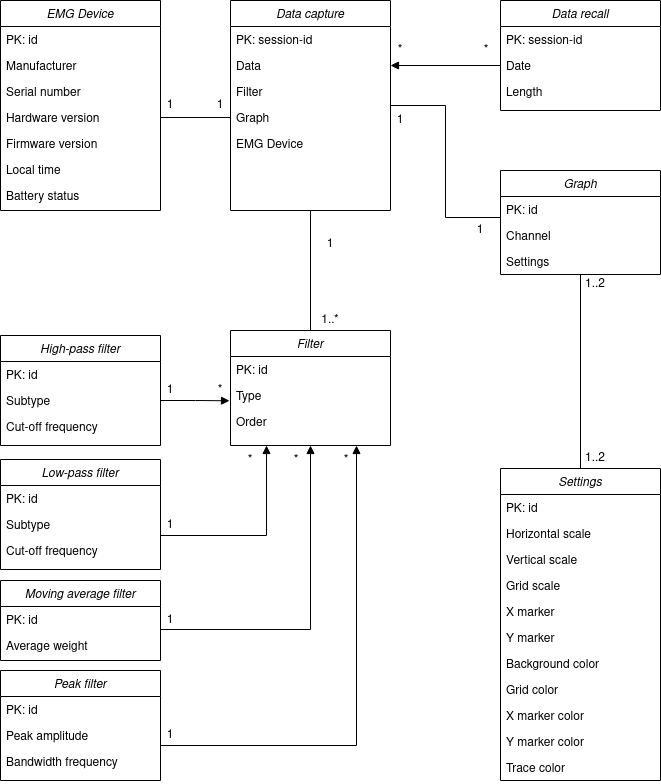
\includegraphics[scale=0.50]{Project Data Classes.png}
	\caption{Data Classes}
	\label{Data Classes}
\end{figure}

\newpage

\section{Requirements Testing}

\subsection{Coverage Table}

\begin{table}[htbp]
	\centering
	
	\begin{tabular}{|l|l|l|l|}
		\hline
		\textbf{Req\#} & \textbf{Description} & \textbf{Coverage} & \textbf{Test method}\\
		\hline
		4.1 & Menu bar & Yes & Manual\\
		\hline
		4.1.1 & Status bar & Yes & Manual \\
		\hline
		4.1.2 & Closing the application & Yes & Manual \\
		\hline
		4.1.3 & Out of range data & Yes & Manual \\
		\hline
		4.2 & Data capture & Yes & Automated \\
		\hline
		4.2.1 & Device connection methods & Yes & Automated \\
		\hline
		4.2.2 & Data capture properties & Yes & Manual \\
		\hline
		4.2.3 & Data capture length & Yes & Automated \\
		\hline
		4.2.4 & Live data capture & Yes & Automated \\
		\hline
		4.2.5 & Data saving & Yes & Automated \\
		\hline
		4.2.6 & Data recall & Yes & Automated \\
		\hline
		4.3 & Filter library & Yes & Automated \\
		\hline
		4.3.1 & Noise filtering & Yes & Automated \\
		\hline
		4.3.2 & Data filtering & Yes & Automated \\
		\hline
		4.4 & Graph settings & Yes & Manual \\
		\hline
		4.4.1 & Data navigation & Yes & Manual \\
		\hline
		4.4.2 & Graph screenshot & Yes & Automated \\
		\hline
		5.1 & Connecting to an EMG device & Yes & Automated \\
		\hline
		5.1.1 & Connection type & Yes & Automated \\
		\hline
		5.1.3 & Retrieving device information & Yes & Automated \\
		\hline
		5.1.3 & Firmware upgrade & Yes & Manual \\
		\hline
		5.1.4 & Date synchronization & Yes & Automated \\
		\hline
		6.1 & User interface & No & See \hyperref[sec:ReqTestJust]{Appendix C} for justification \\
		\hline
		6.1.1 & Application graph & No & See \hyperref[sec:ReqTestJust]{Appendix C} for justification \\
		\hline
		6.1.2 & Touch intuitive controls & No & See \hyperref[sec:ReqTestJust]{Appendix C} for justification \\
		\hline
		6.1.3 & Data display & Yes & Manual \\
		\hline
		6.1.4 & Data recall & Yes & Manual \\
		\hline
		6.2 & Device connection & Yes & Manual \\
		\hline
		6.2.1 & Device wireless connection & Yes & Manual \\
		\hline
		6.2.2 & Device unresponsiveness & Yes & Manual \\
		\hline
		6.3 & Standards compliance & Yes & Manual \\
		\hline
	\end{tabular}
	\textbf{\caption { Test coverage }}
\end{table}

\subsection{Automated Tests}

The automated python tests can be found with the following link: \\ \cite{Github} \href{https://github.com/gmarato/3rq3-softreq}{github.com.com/gmarato/3rq3-softreq}

\newpage

\subsection{Manual Tests}

The following requirements will be tested manually:

\begin{table}[htbp]
	\centering
	\begin{tabular}{|c|l|p{3.5in}|p{1in}|}
		\hline
		\textbf{Req\#} & \textbf{Description} & \textbf{Test method}\\
		\hline
		4.1 & Menu bar  & Tested by visual inspection of application\\
		\hline
		4.1.1 & Status bar  & Tested by visual inspection of application \\
		\hline
		4.1.2 & Closing the application  & Tested by visual inspection of application \\
		\hline
		4.1.3 & Out of range data  & Tested by visual inspection of application with a out of range stimulating input to EMG device \\
		\hline
		4.2.2 & Data capture properties  & Tested by visual inspection of application with a stimulating input to EMG device with a signal within the outlined property limits \\
		\hline
		4.4 & Graph settings & Tested by visual inspection of application and tester interaction \\
		\hline
		4.4.1 & Data navigation & Tested by visual inspection of application and tester interaction \\
		\hline
		5.1.3 & Firmware upgrade & Tested by connecting a EMG device with older firmware and observing the upgrade \\
		\hline
		6.1.3 & Data display & Tested by connecting an EMG device and physically timing the interaction with a stopwatch  \\
		\hline
		6.1.4 & Data recall & Tested by connecting an EMG device and physically timing the interaction with a stopwatch \\
		\hline
		6.2 & Device connection & Tested by connecting and EMG device and physically timing the interaction with a stopwatch \\
		\hline
		6.2.1 & Device wireless connection & Tested by connecting an EMG device and physically timing the interaction with a stopwatch. Device can be disconnected using a wireless blocking chamber \\
		\hline
		6.2.2 & Device unresponsiveness & Tested by connecting and EMG device and physically timing the interaction with a stopwatch. Device can be disconnected using a wireless blocking chamber or sudden wired disconnection \\
		\hline
		6.3 & Standards compliance & Tested and certified with an external testing facility like TUV Sud \\
		\hline
	\end{tabular}
	\textbf{\caption { Manual tests }}
\end{table}


\textbf{NOTE:} For time sensitive tests like 6.1.3 and 6.1.4 high speed cameras and stopwatches with milliseconds precision can be employed to facilitate the tests.

\newpage

\begin{flushleft}
\textbf{{\Large Appendix}}
\end{flushleft}
\appendix
\section{Background Research}

My background research is mostly due to my industry experience in the field. However, I heavily referenced \cite{Biometrics} and \cite{Laborie}
to draw some ideas for the most critical features that an EMG capturing application would have. Obviously, graphing is the most important feature
which both of the applications provided by Biometrics and Laborie do. Along with that they offer the ability to customize the graph in terms scale,
colors and ability to add markers for measurements. Additionally, both offered the ability to save the capture data and recall for later analysis 
with optional features of saving a quick image capture of the graph. Another optional feature that each offer is the ability to filter the data using
standard array of filters. I decided to include the basic array of filtering for now, but other types can always be added in later revisions of the application. 

\newpage

\section{Scenarios}

\subsection{Adding a new EMG device}

\subsubsection{Positive Normal}

\begin{enumerate}
	\item User connects to a new EMG device
	\item Application retrieves EMG device information
	\item EMG device confirmed acceptable
	\item Date is synchronized with the device
	\item Device is ready to be used to capture data
\end{enumerate}

\subsubsection{Positive Normal}

\begin{enumerate}
	\item User plugs in device into host computer via USB cable
	\item Application automatically connects to device
	\item Date is synchronized with the device
	\item Device is ready to be used to capture data
\end{enumerate}

\subsubsection{Positive Normal}

\begin{enumerate}
	\item User pairs EMG device with host computer via Bluetooth
	\item Application automatically connects to device
	\item Date is synchronized with the device
	\item Device is ready to be used to capture data
\end{enumerate}

\subsubsection{Postive Abnormal}

\begin{enumerate}
	\item User connects to a new EMG device
	\item Application retrieves EMG device information
	\item EMG device confirmed unacceptable
	\item Error message is displayed that the device is not compatible 
\end{enumerate}

\subsubsection{Postive Abnormal}

\begin{enumerate}
	\item User does not pair EMG device via BT or connect via USB connection
	\item User tries to connect EMG device
	\item After 1 minute of waiting time, the connection times out
	\item Warning message displayed that the device could not be found
\end{enumerate}

\subsubsection{Negative}

\begin{enumerate}
	\item User connects an unsupported EMG device
	\item Application does not recognize EMG device information
	\item Error message is issued to user that device might not be supported
\end{enumerate}

\subsection{Capturing data}

\subsubsection{Positive Normal}

\begin{enumerate}
	\item User clicks on "Start Capture" button
	\item Application triggers the EMG device to start capturing
	\item Application graph is updated with incoming data from EMG device
\end{enumerate}

\subsubsection{Positive Normal}

\begin{enumerate}
	\item User selects filter type from a list
	\item Application applies filter onto the captured data
\end{enumerate}

\subsubsection{Positive Abnormal}

\begin{enumerate}
	\item Application is capturing from EMG device via Bluetooth
	\item A Bluetooth disconnection occurs
	\item Application recovers and reconnects to EMG device
	\item Application continues capturing EMG data
\end{enumerate}

\subsection{Graphing data}

\subsubsection{Positive Normal}

\begin{enumerate}
	\item User starts capturing data from EMG device
	\item Application starts displaying data on the graph
	\item User adjusts the graph vertical and horizontal scales
	\item User adds markers to the graph
	\item Data is captured up to 1 hour in length
\end{enumerate}

\subsection{Saving and recalling data}

\subsubsection{Positive Normal}

\begin{enumerate}
	\item After a capture user saves data onto local disk
	\item Application saves data in (.csv) format onto disk
\end{enumerate}

\subsubsection{Positive Normal}

\begin{enumerate}
	\item User recalls saved data set from local disk
	\item Graph is populated with data in channel 1
	\item User recalls another saved data set from local disk
	\item Graph is populated with data in channel 2
\end{enumerate}

\subsubsection{Negative}

\begin{enumerate}
	\item User tries to open a file format different than (.csv)  
\end{enumerate}

\newpage

\section{Requirements Test Justification}
\label{sec:ReqTestJust}

The following requirements can not be tested either via automated means or manually:

\begin{table}[htbp]
	\centering
	\begin{tabular}{|c|l|p{3.5in}|p{1in}|}
		\hline
		\textbf{Req\#} & \textbf{Description} & \textbf{Test method}\\
		\hline
		6.1 & User interface  & Cannot be tested as this is a subjective feature. 
								However, several potential users could be called in for a trial test for feedback. 
								Further adjustments can be made if a clinical study is organized and after the application is on market and user feedback is gathered.\\
		\hline
		6.1.1 & Application graph  & Cannot be tested as this is a subjective feature. 
										However, several potential users could be called in for a trial test for feedback. 
										Further adjustments can be made if a clinical study is organized and after the application is on market and user feedback is gathered.\\
		\hline
		6.1.2 & Touch intuitive controls  & Cannot be tested as this is a subjective feature. 
											However, several potential users could be called in for a trial test for feedback. 
											Further adjustments can be made if a clinical study is organized and after the application is on market and user feedback is gathered.\\
		\hline
	\end{tabular}
	\textbf{\caption {  Requirements test justification }}
\end{table}

\newpage
\begin{thebibliography}{9}

\bibitem{Biometrics}
  Biometrics Ltd,
  \textit{“Biometrics Analysis software.”},
  Accessed 2020-10-28,
  www.biometricsltd.com/emg-software
  
\bibitem{Laborie}
  Laborie Medical Technologies,
  \textit{“NXT is modern urodynamics”},
  Accessed 2020-10-28,
  www.laborie.com/experiencenxtpro/

\bibitem{Mayo Clinic}
  Mayo Clinic,
  \textit{“Electromyography (EMG) Test procedure”},
  Accessed 2020-11-18,
  www.mayoclinic.org/tests-procedures/emg/about/pac-20393913

\bibitem{ICGC}
  Laborie Medical Technologies,
  \textit{“Canadian Table of Frequency Allocations”},
  Accessed 2020-11-18,
  www.ic.gc.ca/eic/site/smt-gst.nsf/eng/sf10759

\bibitem{Github}
  Marato Gebremichael,
  \textit{“3rq3-softreq github page”},
  www.github.com/gmarato/3rq3-softreq
 
\end{thebibliography}

\end{document}